\section*{Problema 1}
\textbf{Escribir un programa que genere una caminata aleatoria en una matri de 10x10. El arreglo debe contener inicialmente puntos ``.", y debe recorrers basado en el residuo de un número aleatoria (usar srand y rand()) cuyos resultado puede ser \{0 (arriba), 1 (abajo), 2 (izq), 3 (der)\}, que indican la dirección a moverse. A) Verificar que el movimiento no se salga del arreglo de la matriz, y B) No se pued visitar el mismo lugar más de una vez. Si alguna de estas condiciones intentar moverse hacia otra dirección; si todas las posiciones están ocupadas, finalizar el programa e imprimi el resultado.}

Para este problema se definidio como una constante global el tamaño de la matriz y el maximo de letras posibles. Los valores son 10 y 26 respectivamente. Esto porque existen 26 letras en el código ascii ignorando a la letra ñ. El estado inicial de la matriz contiene unicamente puntos, esto puede verse en la figura \ref{fig:initial_state_problem1}. El programa inicia de dos maneras diferentes, un usuario introduce un punto inicial donde comenzará la caminata o este es escogido aleatoriamente.

\begin{figure}[H]
    \centering
    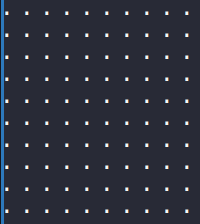
\includegraphics[width=4cm]{Graphics/initial_problem1.png}
    \caption{Estado inicial de la matriz}
    \label{fig:initial_state_problem1}
\end{figure}

Una casilla se considera disponible si su valor es igual a ``.". Antes de obtener el siguiente paso de cada iteracion el programa verifica si sus vecinos estan disponibles. Si existe al menos una casilla disponible entonces el programa sigue (figura \ref{fig:example_walk}), si no el programa termina ya que no podra seguir la caminata (figura \ref{fig:example_block}). El siguinte paso de la iteración se obtiene con la función \textit{rand()}. Se calcula el modulo del número obtenido con 4. Con esto nos aseguramos que el número se encuentre en el conjunto $\{0, 1, 2 ,3\}$.
\begin{center}
    \begin{minipage}{0.48\linewidth}
        \begin{figure}[H]
            \centering
            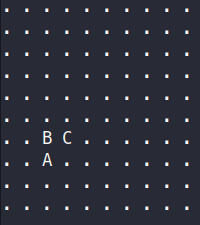
\includegraphics[width=4cm,height=4cm]{Graphics/example_2_1_problem1.png}
            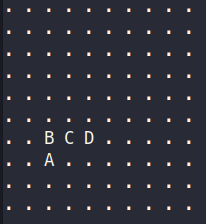
\includegraphics[width=4cm,height=4cm]{Graphics/example_2_2_problem1.png}
            \caption{Ejemplo de caminata.}
            \label{fig:example_walk}
        \end{figure}
    \end{minipage}
    \begin{minipage}{0.48\linewidth}
        \begin{figure}[H]
            \centering
            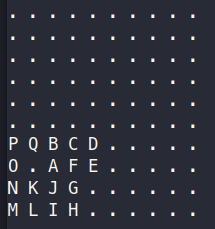
\includegraphics[width=4cm,height=4cm]{Graphics/example_3_1_problem1.png}
            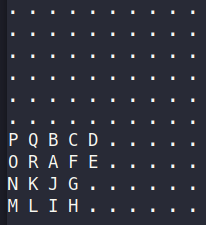
\includegraphics[width=4cm,height=4cm]{Graphics/example_3_2_problem1.png}
            \caption{Ejemplo de termino del programa.}
            \label{fig:example_block}
        \end{figure}
    \end{minipage}
\end{center}

Cada paso debe estar contenido dentro del arreglo de 10x10, si el paso sobrepasa la barrera este es rechazado y se calcula otro diferente. Esto es realizado con la función \textcolor{citecolor}{is\_in\_the\_box} con el siguiente algoritmo:

\begin{lstlisting}[style=CStyle]
    int is_in_the_box(int pos[])
    {
    for (int i = 0; i < 2; i++)
    {
        if ((pos[i] < 0) || (pos[i] >= size))
        {
            return 0;
        }
    }
    return 1;
    }
\end{lstlisting}
Si esta dentro de los límites la función devuelve 1, si esta fuera 0. En la figura \ref{fig:example_final_problema1} se muestran diferentes resultados obtenidos por el programa:

\begin{figure}[H]
    \centering
    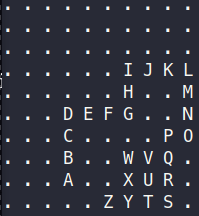
\includegraphics[width=4cm,height=4cm]{Graphics/example_4_1_problem1.png}
    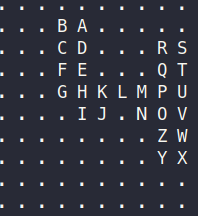
\includegraphics[width=4cm,height=4cm]{Graphics/example_4_2_problem1.png}
    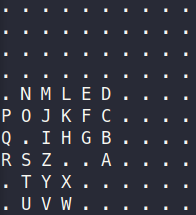
\includegraphics[width=4cm,height=4cm]{Graphics/example_4_3_problem1.png}
    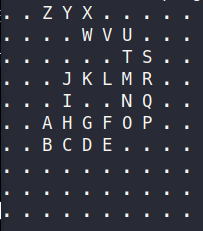
\includegraphics[width=4cm,height=4cm]{Graphics/example_4_4_problem1.png}
    \caption{Diferentes output del programa}
    \label{fig:example_final_problema1}
\end{figure}

El programa se encuentra en la carpeta \textcolor{citecolor}{Problema\_1}. Para compilar el programa se uso el siguiente comando:
\begin{lstlisting}[language=bash]
    gcc -Wall -Wextra -Werror -pedantic -ansi -o main.out main.c -std=c11
\end{lstlisting}
